\documentclass[sigconf]{acmart}

\usepackage{tabularx}
\usepackage{subcaption}
\usepackage{multirow}
\usepackage{hyperref}
%% \BibTeX command to typeset BibTeX logo in the docs
\AtBeginDocument{%
  \providecommand\BibTeX{{%
    Bib\TeX}}}
\def\@copyrightspace{\relax}
\settopmatter{printacmref=false}
\setcopyright{none}
\begin{document}

\title{Testing with Intelligent Transportation Systems and Smart Mobility Schemes\\}

\author{David Fang}
\email{up202004179@up.pt}
\affiliation{%
  \institution{Faculty of Engineering, University of Porto}
  \city{Porto}
  \country{Portugal}
}

\author{Mariana Rocha}
\email{up202004656@edu.fe.up.pt}
\affiliation{%
  \institution{Faculty of Engineering, University of Porto}
  \city{Porto}
  \country{Portugal}
}


\author{Pedro Correia}
\email{up202006199@edu.fe.up.pt}
\affiliation{%
  \institution{Faculty of Engineering, University of Porto}
  \city{Porto}
  \country{Portugal}
}

\begin{abstract}
This work investigates different traffic management settings on intersections to understand which adjustments have major impact on the traffic flow, improving or degrading it.  By leveraging modelling and simulation, using NetLogo, four major scenarios are tested with different settings and the data, collected under the same conditions in all of the different scenarios is analyzed to understand the metrics that can create the optimal system.
\end{abstract}

\keywords{Modelling, System Modelling, Intersections, Traffic Management, Smart City, NetLogo}


\maketitle



\section{Introduction}
Traffic congestion has become a significant challenge in urban areas, contributing to delays, environmental degradation \cite{zhangAirPollutionHealth2013}, and commuter frustration 
\cite{liInfluenceTrafficCongestion2020}. Traditional traffic control systems, which often rely on static or pre-programmed signal timings, are inadequate for managing the dynamic and fluctuating nature of traffic flow. To address this issue, this project explores the use of a simulation model where traffic signals are managed by a Multi-Agent System (MAS). These autonomous agents dynamically adapt to changing traffic conditions, ensuring more efficient and equitable traffic flow across a network of intersections. 
This report details the simulation problem, the model’s design, implementation details, results, and conclusions.

\section{Simulation Problem}

The project’s primary goal is to implement a simulation where several traffic signal control strategies are explored, with multi-agent being one of them. Additionally, the system seeks to balance efficiency and fairness, ensuring that no single route or intersection experiences disproportionately high delays.
Furthermore, the concept of priority vehicles is introduced to mimic vehicles such as ambulances, fire trucks, or police cars. These vehicles need to make it to their destinations quickly to respond to emergencies and ensure public safety. 

\section{Simulation Model}

The simulation model is designed to dynamically represent the complexities of urban traffic systems. It provides a detailed framework for analyzing how traffic signals can adapt to varying conditions to improve overall flow. By implementing speculative modeling techniques, the system allows for the exploration of multiple scenarios. This methodology also includes a variety of strategies that allow the system to respond to real-time data, which includes variables such as traffic density and delays in vehicle movement. The model emphasizes the interconnected nature of intersections and the importance of coordinated adjustments to minimize bottlenecks and congestion.

\subsection{Main Entities}

The simulation encompasses the following entities:
\begin{itemize}
    \item \textbf{Traffic Signals (Agents):} Each traffic signal operates as an autonomous agent capable of making decisions based on localized data and/or information exchanged with neighboring signals. These agents dynamically adjust light timings to optimize traffic flow at their respective intersections.
    \item \textbf{Vehicles:} Represented as individual entities navigating through the network, vehicles adhere to traffic rules and interact with signals. Their movements and delays are tracked to measure the system's efficiency.
    \item \textbf{Intersections:} Critical junctions where multiple roads converge, containing a traffic signal for each road.
    \item \textbf{Roads:}  The network of streets connecting intersections,  serving as pathways for vehicles to spawn and move.
\end{itemize}

\subsection{System Variables}
\label{variables}

The model contains several exogenous variables that allow for the customization and testing of different scenarios, allowing for a detailed exploration of traffic control strategies:


\begin{itemize}
    \item \textbf{Grid Size X and Y:} Specifies the dimensions of the road network in terms of the number of intersections along the X and Y axes.
    \item \textbf{Speed Limit of Vehicles:} Specifies the maximum allowable speed for vehicles on various road segments.
    \item \textbf{Maximum Acceleration:} Determines the highest acceleration rate for vehicles.
    \item \textbf{Maximum Braking Capacity:} Reflects the maximum deceleration rate.
    \item \textbf{Frequency of Cars from North and West:} Controls the rate at which vehicles enter the network from different directions, simulating varied traffic demand patterns.
    \item \textbf{Green Light Length:} Represents the duration of green signals.
    \item \textbf{Yellow Light Length:} Specifies the duration of the yellow light.
    \item \textbf{Weights for Priority Score Calculation:} Factors such as vehicle density, waiting time, and the number of priority vehicles on a road segment contribute to a calculated score used to determine signal timings. These weights are tuned to balance the efficiency-fairness trade-off.
\end{itemize}

The model also includes several endogenous variables, which are generated within the system and reflect its dynamic behavior:

\begin{itemize}
    \item \textbf{Traffic Density:} Indicates the number of vehicles on a specific road segment at any given moment, aiding in identifying congestion hotspots.
    \item \textbf{Vehicle Waiting Time:} Tracks the cumulative time vehicles spend waiting at red lights, directly affecting system efficiency and user satisfaction.
    \item \textbf{Input Traffic Volume:} The number of vehicles entering the system from various directions during a specified period.
    \item \textbf{Output Traffic Volume:} The number of vehicles exiting the system after passing through the intersections.
    \item \textbf{Number of Accidents:} Tracks collision occurrences within the network, providing insights into system safety.
    \item \textbf{Number of Priority Vehicles:} Reflects the count of emergency or public service vehicles within the network.
    \item \textbf{Waiting Time for Priority Vehicles:} Monitors the delays experienced by priority vehicles, essential for evaluating the effectiveness of priority-based strategies.
\end{itemize}

\subsection{Operation Policies}

The system evaluates multiple traffic control policies to determine their effectiveness under varying conditions:
\begin{itemize}
    \item \textbf{Fixed-Time Control}: A traditional approach where signal timings are predefined and do not adapt to real-time conditions. While simple to implement, this policy often leads to inefficiencies during peak traffic.
    \item \textbf{Adaptive Traffic Signal Control}: This policy adjusts signal timings dynamically based on real-time traffic data, such as vehicle density, waiting times, and a road priority score explained in more detail in section(secção futura).
    \item \textbf{Multi-Agent System (MAS) Control:} In this advanced approach, traffic signals operate as independent agents that not only manage their own intersection but also coordinate with signals at neighboring intersections to optimize traffic flow collaboratively.
    \item \textbf{Priority-Based Control:} Designed to prioritize certain types of vehicles, such as emergency services and public transport. While effective for specific goals, this policy requires balancing the needs of regular traffic to prevent significant delays.
    \item 
\end{itemize}

\subsection{Performance Metrics}
The effectiveness of the system is evaluated using the following metrics:
\begin{itemize}
    \item \textbf{Average Vehicle Waiting Time:} Reflects the mean delay experienced by vehicles at intersections, serving as a primary indicator of traffic flow efficiency.
    \item \textbf{Input Traffic Volume:} The number of vehicles that entered the system from various directions during the specified period.
    \item \textbf{Output Traffic Volume:} The number of vehicles that exited the system during the specified period.
    \item \textbf{Number of Accidents:} The number of accidents that occurred during the simulation.
    \item \textbf{Priority Vehicle Waiting Time:}  Reflects the mean delay experienced by priority vehicles at intersections.
\end{itemize}

\section{Implementation Details}
The simulation’s implementation leveraged NetLogo, a multi-agent programmable modeling environment, for its simplicity and suitability for traffic management research. Python was also used to connect with NetLogo and run different experiments with varied input parameters. Together, these tools enabled the development of a speculative model to simulate and evaluate various scenarios.

\subsection{NetLogo}

Before running the simulation, preparations need to be made. This includes setting up the exogenous variables referred in section \ref{variables}, and the operation policy to be tested. To do that, we have the switches and the sliders shown in Fig. \ref{fig:setup}.

\begin{figure}
    \centering
    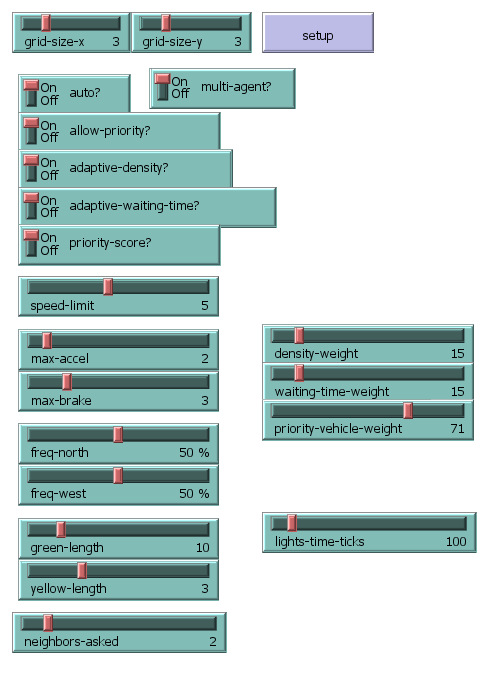
\includegraphics[width=1\linewidth]{images/netlogo.png}
    \caption{Setup: Switches and Sliders}
    \label{fig:setup}
\end{figure}

Below is a brief description of each switch and slider:
\begin{itemize}
    \item \textbf{grid-size-x:} Defines the number of roads on the x-axis.
    \item \textbf{grid-size-y:} Defines the number of roads on the y-axis.
    \item \textbf{setup:} Initializes the simulation.
    \item \textbf{auto?:} Toggles the fixed-time control strategy on or off.
    \item \textbf{multi-agent?:} Toggles the multi-agent mode on or off.
    \item \textbf{allow-priority?:} Allows or disallows the priority-based control strategy in the simulation. Should only be activated along the auto? switch.
    \item \textbf{adaptive-density?:} Enables or disables adaptive strategy that relies on the traffic density.
    \item \textbf{adaptive-waiting-time?:} Enables or disables adaptive strategy that relies on the vehicles’ waiting time.
    \item \textbf{priority-score?:} Enables or disables adaptive strategy that relies on the road priority score.
    \item \textbf{speed-limit:} Controls the speed limit in the simulation.
    \item \textbf{max-accel:} Controls the vehicle’s maximum acceleration.
    \item \textbf{max-brake:} Controls the vehicle’s maximum braking force.
    \item \textbf{freq-north:} Controls the frequency of vehicles coming from the north.
    \item \textbf{freq-west:} Controls the frequency of vehicles coming from the west.
    \item \textbf{green-length:} Controls the length of the green light.
    \item \textbf{yellow-length:} Controls the length of the yellow light.
    \item \textbf{neighbors-asked:} Controls the number of neighboring agents asked.
    \item \textbf{density-weight:} Controls the weight of density in the simulation. It's crucial that the total of these weights equals 100 for normalization purposes.
    \item \textbf{waiting-time-weight:} Controls the weight of waiting time.
    \item \textbf{priority-vehicle-weight:} Controls the weight of priority vehicles.
    \item \textbf{lights-time-ticks:} Controls the amount of ticks it takes to store the average waiting time of a light during those x amount of ticks. Only used to analyse the behavior of the lights, doesn’t affect the final results.
\end{itemize}

Once everything is set up correctly, clicking on setup will display Figure x+1 on the screen. The user can then run the model by either clicking the go button to run the simulation automatically, or the go-once button to run the simulation one tick at a time.

\begin{figure}
    \centering
    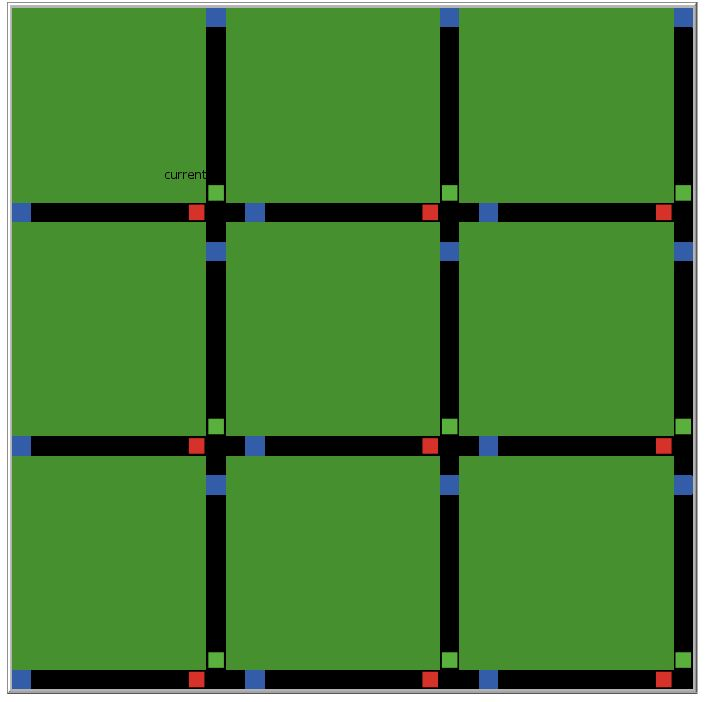
\includegraphics[width=1\linewidth]{images/netlogogrid.JPG}
    \caption{Netlogo grid}
    \label{fig:Netlogo grid}
\end{figure}

To attach the scenarios referenced at the section X, several strategies were implemented and handled by the following variables.

\subsubsection{auto?}
In this strategy, the traffic signals change based on the values of the green-length and yellow-length variables. There is no need for a separate red length, as once a light finishes its green phase and switches to yellow, the other traffic signal automatically changes from red to green.

\subsubsection{adaptive-density?}
This strategy dynamically adjusts traffic light signals based on the current traffic density on each road. It compares the density of vehicles on each road at an intersection and prioritizes the road with higher traffic density by turning its signal green. Density is calculated by the difference between the traffic output of a traffic signal and its input. Input refers to the number of cars that reach the traffic signal, while output refers to the number of cars that pass through it. This helps to alleviate congestion by allowing more vehicles to pass through the intersection from the busier road.

\subsubsection{adaptive-waiting-time?}
This strategy focuses on minimizing waiting times for vehicles at an intersection. It continuously monitors the waiting time for vehicles on each road and prioritizes the road with the longest waiting time by turning its signal green. This ensures that vehicles do not remain stationary for extended periods, improving overall traffic flow and reducing delays.

\subsubsection{priority-score?}
This strategy combines elements of both the adaptive-density and adaptive-waiting-time strategies, as well as incorporating priority for special vehicles. It calculates a priority score for each road at an intersection based on factors such as traffic density, waiting time, and the presence of priority vehicles. The priority score is calculated by the following formula.

\[
 RPS_R = W_1 \cdot D_R + W_2 \cdot W_R + W_3 \cdot P_R
\]
Where: 
\textit{
\begin{itemize}
    \item RPS is the Road Priority Score
    \item R represents the road
    \item D is the density
    \item T is the waiting time
    \item P is the amount of priority vehicles
    \item W is the weight of the variable.
\end{itemize}
}

 The road with the highest priority score is given the green signal, optimizing the intersection's overall efficiency and accommodating different traffic conditions.

\subsubsection{multi-agent?}
This strategy utilizes a Global Priority Score (GPS) to manage traffic flow across multiple intersections. Each intersection calculates its priority score based on factors such as traffic density, waiting time, and the presence of priority vehicles. The Global Priority Score for each intersection is determined by considering the priority score of the intersection itself and those of its neighboring intersections to the left and top adjusted by their distance since, in our setup, vehicles only travel from north to south or from west to east. This ensures a coordinated approach to traffic management across the network, allowing intersections to prioritize based on a broader understanding of traffic conditions. This decentralized, yet coordinated strategy aims to optimize overall traffic flow and minimize delays by dynamically responding to real-time changes in traffic conditions. The GPS formula is represented below:

\[
\text{GPS}_R = \sum_{R \in I} \text{RPS}_R \cdot \frac{1}{D_I}
\]

Where: 
\textit{
\begin{itemize}
    \item R represents the road of the same direction
    \item RPS is the road priority score
    \item D is the distance
    \item I represents the intersection
\end{itemize}
}


The simulation also allows users to manipulate traffic light settings and select specific intersections for monitoring. The buttons in Figure \ref{fig:controls} enable the user to manage traffic flow and observe the effects of their changes in real time.

\begin{itemize}
    \item \textbf{Switch All Lights:} This button allows the user to switch all traffic lights at the intersections.
    \item \textbf{Switch Current Light:} This button enables the user to switch the traffic light at the currently selected intersection.
    \item \textbf{Select Intersection:} This button lets the user choose a specific intersection to monitor. The selected intersection's data will be reflected in the corresponding graphs and monitors.
\end{itemize}

\begin{figure}
    \centering
    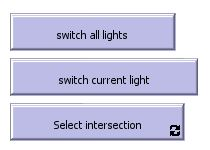
\includegraphics[width=0.5\linewidth]{images/netlogoCurrent.JPG}
    \caption{Interactive Controls}
    \label{fig:controls}
\end{figure}

NetLogo provides several visualization tools to monitor and analyze traffic data at an intersection. Figure x+2 shows various monitors and graphs that track different aspects of traffic flow and waiting times. 

\begin{figure}
    \centering
    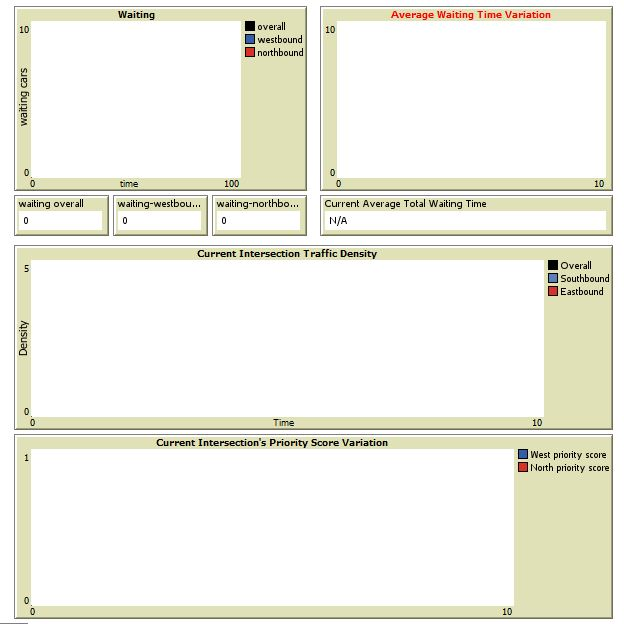
\includegraphics[width=1\linewidth]{images/netlogomonitors2.JPG}
    \caption{Netlogo Monitors}
    \label{fig:monitors1}
\end{figure}

\begin{figure}
    \centering
    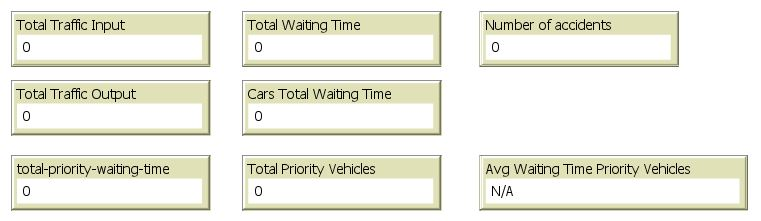
\includegraphics[width=1\linewidth]{images/netlogomonitors1.JPG}
    \caption{More Netlogo Monitors}
    \label{fig:monitors2}
\end{figure}

Here are the descriptions for each monitor:
\begin{itemize}
    \item \textbf{Waiting:} This graph displays the number of vehicles waiting in three categories: overall, westbound, and northbound. The x-axis represents time, and the y-axis represents the number of waiting cars.
    \item \textbf{Average Waiting Time Variation:} This graph shows the variation in average waiting times over a period. The x-axis represents time, and the y-axis represents the waiting time.
    \item \textbf{Current Average Total Waiting Time:} This monitor displays the current average total waiting time for vehicles.
    \item \textbf{Current Intersection Traffic Density:} This graph shows the traffic density at the current selected intersection for three categories: overall, southbound, and eastbound. The x-axis represents time, and the y-axis represents density.
    \item \textbf{Current Intersection's Priority Score Variation:} This graph displays the variation in the currency selected intersection's priority score for west and north directions. The x-axis represents time, and the y-axis represents the priority score.
    \item \textbf{Total Traffic Input:} This monitor shows the total number of vehicles entering the network of intersections.
    \item \textbf{Total Waiting Time:} This monitor displays the total waiting time for all vehicles.
    \item \textbf{Number of Accidents:} This monitor shows the total number of accidents that have occurred.
    \item \textbf{Total Traffic Output:} This monitor displays the total number of vehicles that left the network of intersections.
    \item \textbf{Cars Total Waiting Time:} This monitor shows the total waiting time for the current cars in the network.
    \item \textbf{Total Priority Waiting Time:} This monitor displays the total waiting time for priority vehicles.
    \item \textbf{Total Priority Vehicles:} This monitor shows the total number of priority vehicles that appeared in the network.
    \item \textbf{Avg Waiting Time Priority Vehicles:} This monitor displays the average waiting time for priority vehicles.
\end{itemize}

\subsection{Python}
To facilitate the evaluation of various traffic light strategies and parameters, a Python script, model.py, was developed to interface with the NetLogo model. This script automates the process of running the simulation with different configurations and collects performance metrics for analysis. Here’s an overview of how it works:

It first establishes a connection with the NetLogo model and prompts the user to input values such as the grid size and vehicle frequency. These values are then set within the NetLogo model to customize the simulation setup.

The script then defines a list of default states to reset the model’s switches to a baseline configuration before each simulation run. It specifies various parameters that will be tested, including the lengths of green and yellow traffic light phases, the number of neighboring intersections considered, and weights for priority score calculations. Valid weight combinations are generated to ensure that the sum of these weights equals 100, maintaining normalization and consistency in the priority scoring system.

Finally, the script iterates through various traffic light strategies and parameter combinations, running the model for 10000 ticks for each configuration. It systematically tests each strategy, adjusting parameters as needed and storing the results for further analysis. By doing so, the script provides a comprehensive evaluation of different traffic management strategies under various conditions. The collected results are then saved to a file for further analysis.

\section{Main Results and Discussion}

To compare the different strategies, the model.py file was run with a 3x3 grid size and a 50\% frequency for both the north and west directions. For the adaptive models, adaptive-density and adaptive-waiting, only the priority score was used, as using the maximum weight on density or waiting time effectively represents both models. To ensure the evaluation was robust and repeatable, a fixed random seed (e.g., random-seed 42) was set. This guaranteed that the random vehicle spawning function produced the same positions across all runs.

\subsection{Total Traffic Input \& Total Traffic Output}

The \textbf{Allow Priority Model} shows a median traffic output of 9871.00 [ Table \ref{tab:tab1}], indicating that most scenarios achieve high output. However, the average output is lower at 8433.66, driven down by significant outliers such as the extremely low minimum output (27.00). This discrepancy between the median and the average, along with the high variability (SD = 3469.62), suggests that while the model performs well in typical scenarios, it struggles with extreme cases. Similarly, for traffic input, the median is 9906.50 [ Table \ref{tab:tab1}], but the lower average of 8476.96 reflects inconsistencies caused by large outliers, as evidenced by the minimum input (108.00).

The \textbf{Auto Model} demonstrates exceptional consistency, with a median traffic output of 9910.00 and an average of 9853.17, which are closely aligned. This alignment, along with minimal variability (SD = 331.87), shows that the model performs consistently across scenarios. The input statistics further reinforce this reliability, with a median of 9935.00 and an average of 9879.22, both indicating consistent handling of traffic volumes with minimal impact from outliers.

The \textbf{Multi-Agent Model} achieves a balanced approach, with a median traffic output of 9875.50 and an average of 8763.06. The gap between these values, combined with a significant variability (SD = 1904.50), suggests that the model generally performs well but can underperform in some scenarios, as reflected in its minimum output (1670.00). Similarly, for input, the median is 9924.01, slightly higher than the average of 8827.84, indicating occasional inefficiencies in managing traffic inflow.

The \textbf{Priority Score Model} has a median traffic output of 9891.00, slightly higher than the average of 7822.98, highlighting a strong influence from outliers. The large variability (SD = 2876.57) and the low minimum output (2575.00) reinforce this inconsistency. For input, the median is 9939.02, higher than the average of 7900.64, which also points to significant outliers affecting the overall performance.

\subsection{Waiting Times}

The \textbf{Allow Priority Model} exhibits the highest average waiting times among all the strategies analyzed, with general traffic experiencing an average wait of 614.88 ticks [Table \ref{tab:tab3}] and a standard deviation (SD) of 1620.32. This indicates not only inefficiency in managing traffic flow but also significant variability in its performance. The median waiting time for general traffic is 22.35 ticks, which is considerably lower than the average, suggesting that most vehicles face shorter waiting times, but extreme outliers affect the results. For priority vehicles, the situation improves slightly, with an average waiting time of 390.25 ticks and a median of 3.86 ticks [Table \ref{tab:tab5}], highlighting the model's intention to prioritize these vehicles effectively in most cases. However, the variability remains high (SD = 1084.39), reflecting inconsistent performance. While the model succeeds in reducing waiting times for the majority of priority vehicles, its inability to manage extreme scenarios restricts its overall effectiveness.

The \textbf{Auto Model} achieved the lowest average waiting time for general traffic at 17.49 ticks, accompanied by low variability (SD = 13.85). This reflects a consistent performance in managing traffic flow. The median waiting time for general traffic is 13.56 ticks, closely aligned with the average, emphasizing the model's reliability in providing uniform and predictable traffic management. Priority vehicles experience nearly identical results, with an average waiting time of 17.45 ticks, a median of 13.49 ticks, and slightly higher variability (SD = 13.98).

The \textbf{Multi-Agent Model} displayed a balance between efficiency and adaptability. General traffic sees a moderate average waiting time of 55.97 ticks, with relatively low variability (SD = 85.25). The median waiting time for general traffic is 13.14 ticks, highlighting that a majority of vehicles experience minimal delays, although occasional inefficiencies inflate the average. For priority vehicles, the average waiting time is 51.54 ticks, with a median of 11.69 ticks and a similar standard deviation (SD = 86.00). This indicates that the model effectively balances the needs of different types of vehicles while maintaining a consistent level of service. The proximity between average and median values reflects the model's capacity to provide reliable traffic management for both general and priority vehicles, even under varying conditions.

The \textbf{Priority Score Model} demonstrates a higher average waiting time for general traffic at 109.77 ticks, with moderate variability (SD = 157.72). The median waiting time is 9.94 ticks, significantly lower than the average, suggesting that the majority of vehicles experience relatively short delays while outliers contribute to increased overall waiting times. For priority vehicles, the average waiting time decreases slightly to 103.25 ticks, with a median of 8.18 ticks. However, the variability (SD = 161.06) remains comparable to that of general traffic, indicating occasional inefficiencies in handling priority scenarios. This model, which adjusts traffic lights based on real-time data and calculated scores, shows potential for managing specific situations where priority vehicles need to be addressed. However, its higher waiting times and variability suggest a trade-off, where extreme cases are prioritized at the expense of overall consistency. This may limit its effectiveness in environments requiring a more uniform distribution of waiting times.

\subsection{Accidents}

The model that showed the best results regarding accidents was the \textbf{Auto Model}. This is because the fixed schedule avoids all possibilities of conflicts, ensuring that all north-facing lights are green while all west-facing lights are red, and vice versa. This eliminates any chance of collisions, resulting in an average of 0 accidents [Table \ref{tab:tab4}].

The \textbf{Allow Priority Model} also achieves low accident rate values regarding accidents with the average being 1.53 accidents per 10,000 ticks.  This is attributed to its ability to dynamically change the lights at an intersection to allow priority vehicles to pass safely while ensuring the opposing light is red to prevent conflicts. The consistency of its performance is reflected in the low standard deviation (SD =  1.54).

The \textbf{Multi-Agent Model} showed a higher accident rate compared to the simpler models, with an average of 9.81 accidents per 10,000 ticks. The same applies to the \textbf{Priority Score Model}, which also demonstrated a higher accident rate of 10.36 accidents per 10,000 ticks. The Multi-Agent Model relies on multiple agents working together to manage traffic across intersections, to optimize traffic flow through collaborative decision-making. However, its complexity introduces variability, leading to higher average accident numbers. On the other hand, the Priority Score Model changes traffic lights based on real-time data. Despite the real-time adjustments, its complexity still results in higher accident rates compared to the simpler models.
The median of 5.0 in both models suggests that while some settings perform well, others are prone to higher accident rates. This indicates that both models require further refinement to handle diverse traffic scenarios more effectively and consistently

\subsection{Discussion}

The results indicate that the performance of traffic light strategies can vary based on the specific objectives of the analysis. For example, if the primary goal is to maximize traffic output, the \textbf{priority score} model with weights (50, 40, 10) proves to be the most effective. This configuration achieves a traffic output of 10,178, with an average waiting time of 2.89 ticks and a priority average waiting time of 2.58 ticks, however with 15 accidents. In comparison, the \textbf{Multi-Agent} model with the same weights yields a lower traffic output of 9,835. However, it significantly outperforms in terms of average waiting time and priority handling. With one neighbor, the average wait time is 1.09 ticks, and the priority wait time is 0.42 ticks. For two neighbors, these values are 1.08 ticks and 0.47 ticks, respectively. Despite this, the multi-agent model has 22 accidents in both cases, slightly higher than the priority score model. This reminds that even the best case scenarios for some metrics come with less than ideal KPIs for others, such as accident rates or waiting times, emphasizing the need to balance trade-offs based on the analysis objectives.

Another idea to be highlighted is that even though \textbf{Auto} Model exhibits better results on average for waiting times when compared to the \textbf{Priority Score} and the \textbf{Multi-Agent} models, this happens due to the fact that multiple settings are being tested rather than just the optimal ones. The two last models are highly influenced by the weights applied to the priority function, which drastically affect the traffic flow. In contrast, the Auto model setting changes do not cause such extreme changes, leading to more consistent but less optimized waiting times.

The best results or waiting times for both priority and overall vehicles are seen on the \textbf{Priority Score} and \textbf{Multi-Agent} scenarios. These models are capable of dynamically adjusting to traffic conditions, allowing them to improve waiting times based on real time data and further study is required to identify the most effective combinations. 

An important observation is that, while both models achieve a minimum average priority vehicle waiting time of 0 ticks, this outcome is the result of a specific scenario during the simulation rather than true optimal performance. In this case, the weight distribution was set to (0, 0, 100), prioritizing only the passage of priority vehicles. Combined with the selected random seed, this configuration caused priority vehicles to spawn exclusively on vertical roads. As a result, the traffic signals for horizontal roads never changed to green, leaving vehicles on those roads indefinitely stuck. This issue is further evidenced by the significantly reduced traffic input and output values, which are approximately half of the median (around 5,000 vehicles in both cases).

This highlights the critical need to evaluate traffic models not only based on performance estimates but also through direct observation of their behavior during simulations. Such analysis ensures that potential flaws or unrealistic outcomes are identified and addressed before selecting a model for implementation.

To sum up,  different scenarios and objectives might lead to different conclusions. The adaptive-waiting model, while showing overall benefits, may not always be the optimal choice depending on the specific traffic conditions or goals of the traffic management system. Future research should consider a broader range of variables, such as pedestrian traffic and environmental factors, to enhance the robustness and applicability of these models.

\section{Conclusions}

As a speculative model, this simulation offers a flexible framework that can adapt to various needs and use cases. It serves as a foundation for further exploration and refinement in the field of traffic management.

The results of the simulation highlight that the optimal traffic management scenario varies depending on the prioritized metric, as different metrics may lead to different results. This underlines the importance of aligning the chosen scenario with the stakeholders’ specific goals and priorities. The model proves to be an interesting tool in guiding these decisions, providing insights into the trade-offs between different traffic management strategies.


For future work, several paths can be followed to enhance the model's capabilities:
\begin{itemize}
    \item Advanced Algorithms: Investigating more sophisticated algorithms that can deliver more precise results while incorporating a wider array of variables and metrics.
    \item Entity Behaviors: Improving the behaviors of the entities within the simulation to more accurately reflect real-world traffic dynamics.
\end{itemize}

The advancements will contribute to a more realistic simulation model, enabling the development of more effective strategies for urban traffic control.


\bibliographystyle{ACM-Reference-Format}
\bibliography{references}
\clearpage

\appendix



\begin{table*}[]
\centering
\caption{Total Traffic Input Statistics Across Traffic Models}
\label{tab:tab2}
\begin{tabular}{lccccc}
\toprule
\textbf{Model} & \textbf{Average} & \textbf{Median} & \textbf{Standard Deviation} & \textbf{Maximum} & \textbf{Minimum} \\
\midrule
Allow Priority & 8476.96 & 9906.50 & 3450.27 & 10163.00  & 108.00  \\ 
Auto &  9879.22 & 9935.00 & 322.24 & 10175.00  & 7632.00  \\ 
Multi-Agent & 8827.84 & 9924.01 & 1881.56 & 10174.00   & 1751.00 \\ 
Priority Score &  7900.64 & 9939.02 & 2834.68 & 10224.00  & 2721.00  \\ 

\bottomrule
\end{tabular}
\end{table*}


\begin{table*}[]
\centering
\caption{Total Traffic Output Statistics Across Traffic Models}
\label{tab:tab1}
\begin{tabular}{lccccc}
\toprule
\textbf{Model} & \textbf{Average} & \textbf{Median} & \textbf{Standard Deviation} & \textbf{Maximum} & \textbf{Minimum} \\
\midrule
Allow Priority & 8433.66 & 9871.00 & 3469.62 & 10136.00  & 27.00  \\ 
Auto & 9853.17 & 9910.00 & 331.87 &  10159.00 & 7553.00 \\ 
Multi-Agent & 8763.06 & 9875.50 & 1904.50 & 10125.00  & 1670.00 \\ 
Priority Score &  7822.98 & 9891.00 & 2876.57 & 10178.00  &  2575.00 \\ 

\bottomrule
\end{tabular}
\end{table*}


\begin{table*}[]
\centering
\caption{Total Average Waiting Time Statistics Across Traffic Models}
\label{tab:tab3}
\begin{tabular}{lccccc}
\toprule
\textbf{Model} & \textbf{Average} & \textbf{Median} & \textbf{Standard Deviation} & \textbf{Maximum} & \textbf{Minimum} \\
Allow Priority &  614.88 & 22.35 & 1620.32 & 7452.62  & 8.92 \\ 
Auto & 17.49 & 13.56 & 13.85 &  91.52 & 8.79 \\ 
Multi-Agent & 55.97 & 13.14 & 85.25 & 509.06  & 1.03 \\ 
Priority Score &  109.77 &  9.94 & 157.72 & 520.02  &  0.78  \\ 

\bottomrule
\end{tabular}
\end{table*}

\begin{table*}[]
\centering
\caption{Accidents Statistics Across Traffic Models}
\label{tab:tab4}
\begin{tabular}{lccccc}
\toprule
\textbf{Model} & \textbf{Average} & \textbf{Median} & \textbf{Standard Deviation} & \textbf{Maximum} & \textbf{Minimum} \\
\midrule
Allow Priority & 1.53  & 1.00 & 1.54 &  6.00 & 0.00 \\ 
Auto & 0.00  & 0.00 & 0.00  &  0.00  & 0.00 \\ 
Multi-Agent & 9.81 & 5.00 & 11.94 &  63.00  & 0.00  \\ 
Priority Score &  10.36  & 5.00 &  12.74  &  58.00  & 0.00\\ 

\bottomrule
\end{tabular}
\end{table*}

\begin{table*}[]
\centering
\caption{Total Priority Average Waiting Time Statistics Across Traffic Models}
\label{tab:tab5}
\begin{tabular}{lccccc}
\toprule
\textbf{Model} & \textbf{Average} & \textbf{Median} & \textbf{Standard Deviation} & \textbf{Maximum} & \textbf{Minimum} \\
Allow Priority & 390.25  & 3.86  &  1084.39 & 4918.50  & 1.11 \\ 
Auto &  17.45 & 13.49  & 13.98  &  94.41 & 8.20 \\ 
Multi-Agent & 51.54 & 11.69 & 86.00 & 684.67 & 0.00 \\ 
Priority Score & 103.25 & 8.18 & 164.06 & 778.23  & 0.00 \\ 

\bottomrule
\end{tabular}
\end{table*}

\begin{figure*}[]
    \centering
    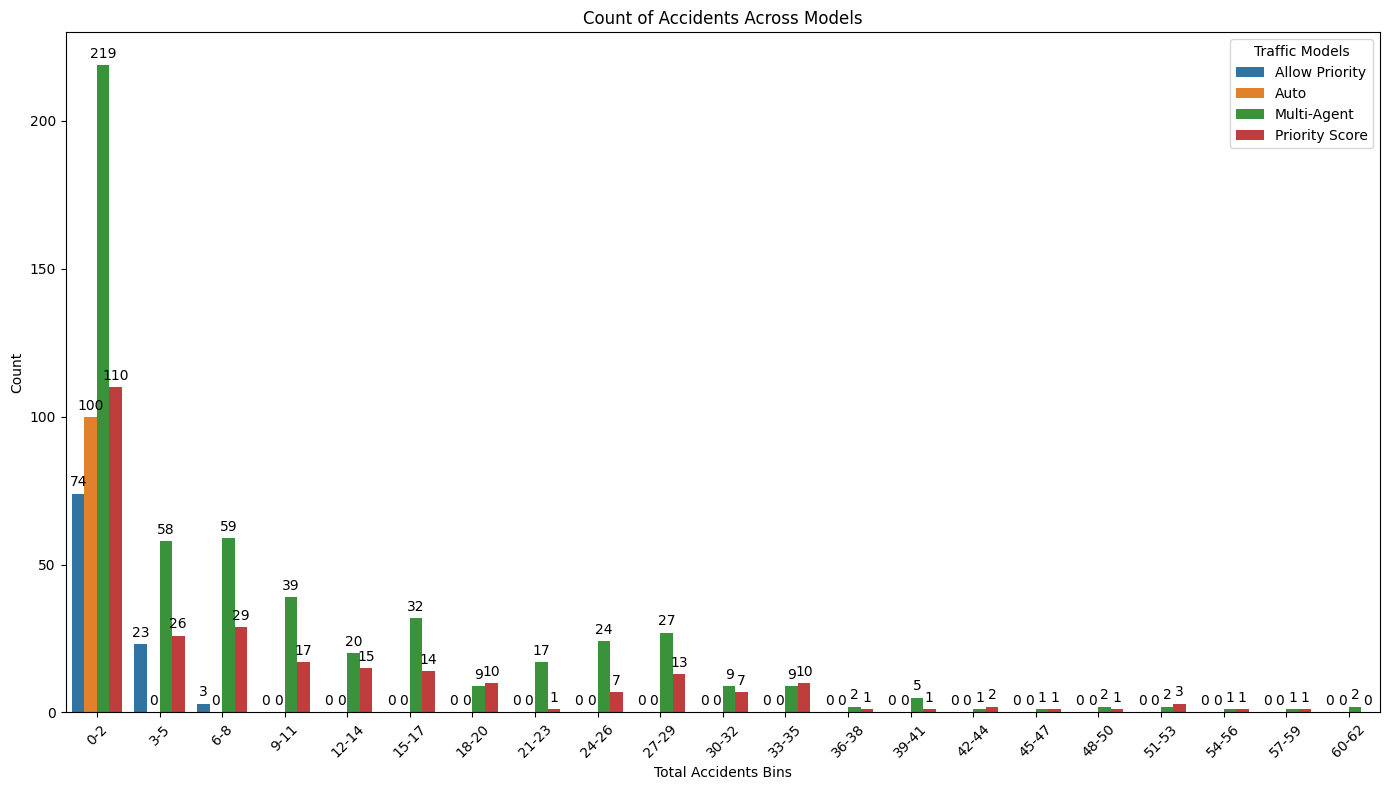
\includegraphics[width=1\linewidth]{images/accidents.png}
    \caption{Total Accidents Count Distribution Across Models}
    \label{fig:pitch-venezuela}
\end{figure*}


\begin{figure*}[]
    \centering
    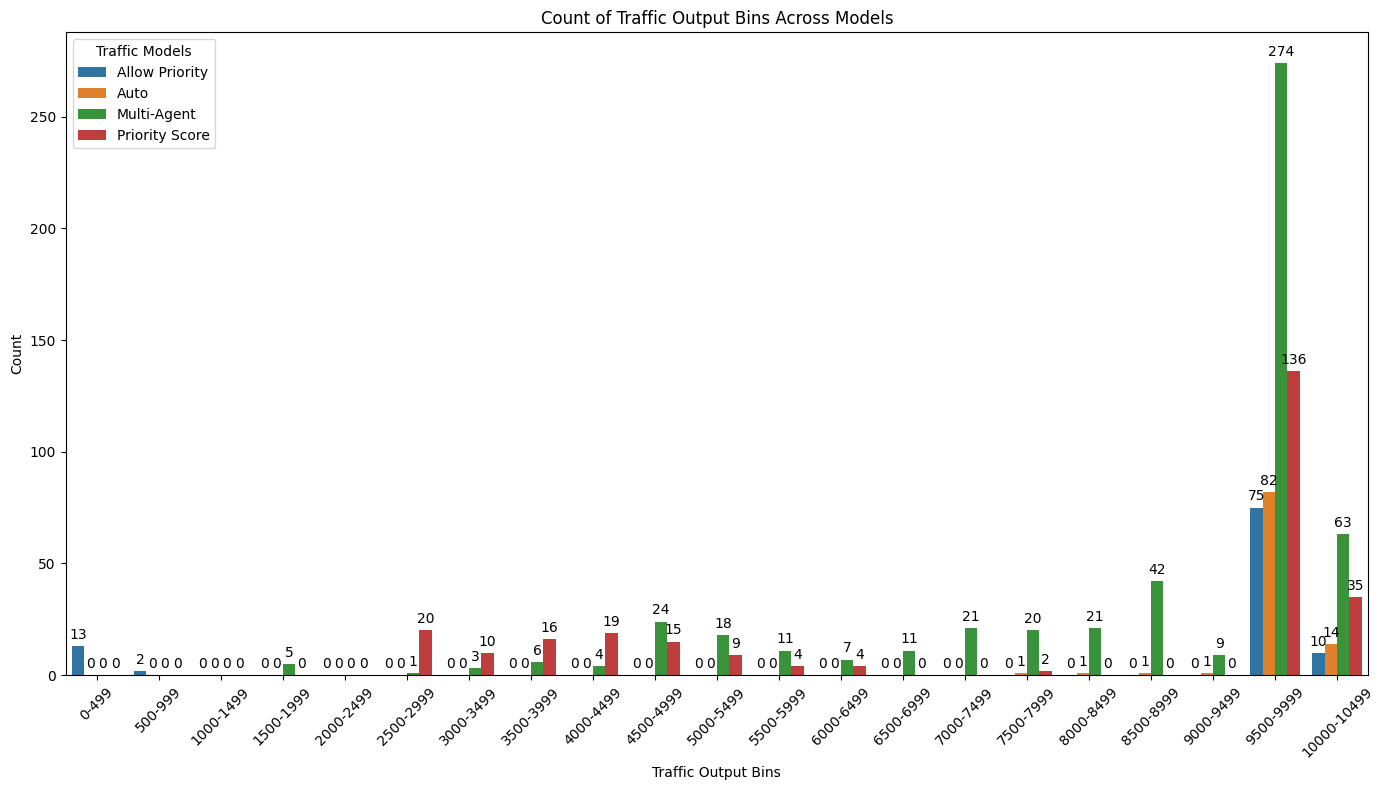
\includegraphics[width=1\linewidth]{images/traffic-output.png}
    \caption{Total Traffic Output Distribution Across Models}
    \label{fig:setup}
\end{figure*}

\begin{figure*}[]
    \centering
    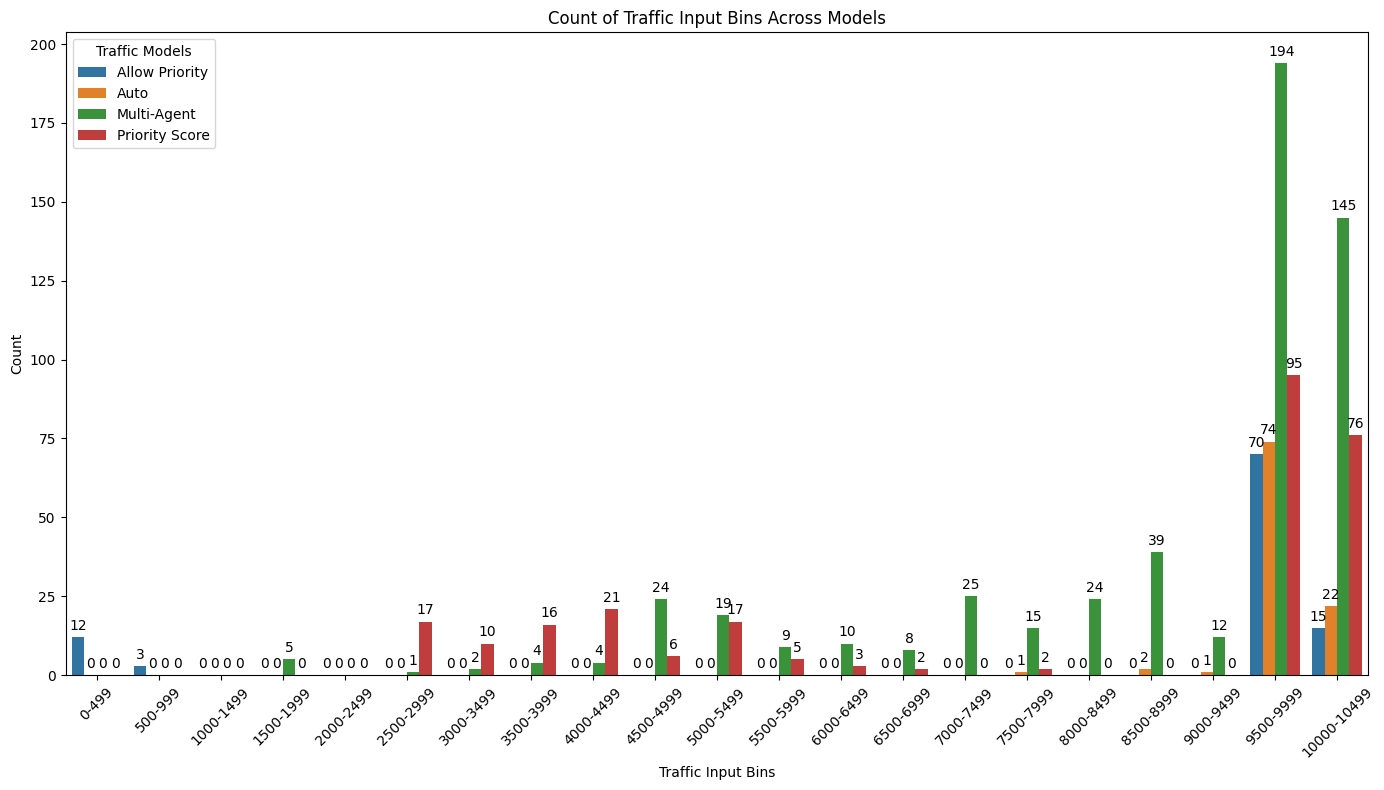
\includegraphics[width=1\linewidth]{images/traffic-input.png}
    \caption{Total Traffic Input Distribution Across Models}
    \label{fig:setup}
\end{figure*}

\begin{figure*}[]
    \centering
    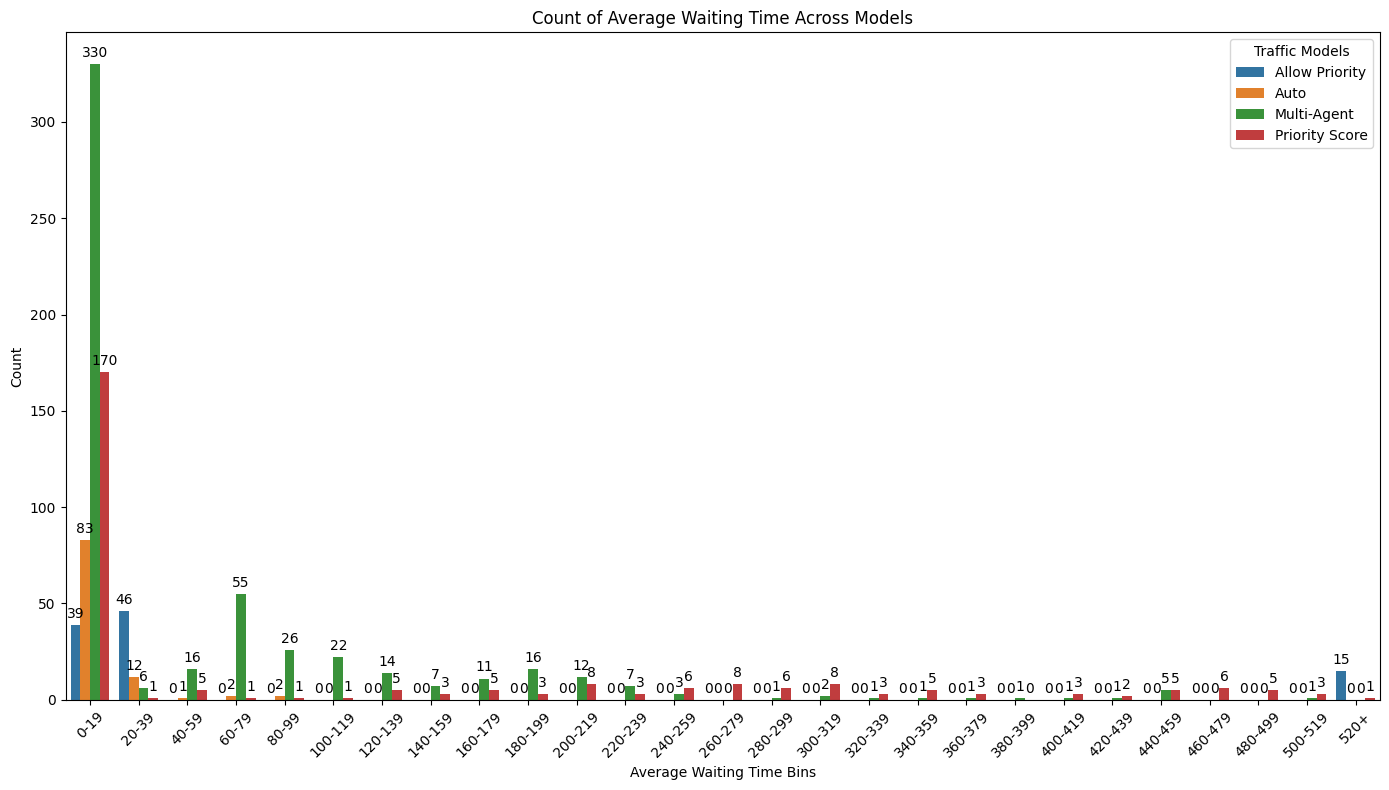
\includegraphics[width=1\linewidth]{images/count-average.png}
    \caption{Average Waiting Time  Distribution Across Models}
    \label{fig:setup}
\end{figure*}


\begin{figure*}[]
    \centering
    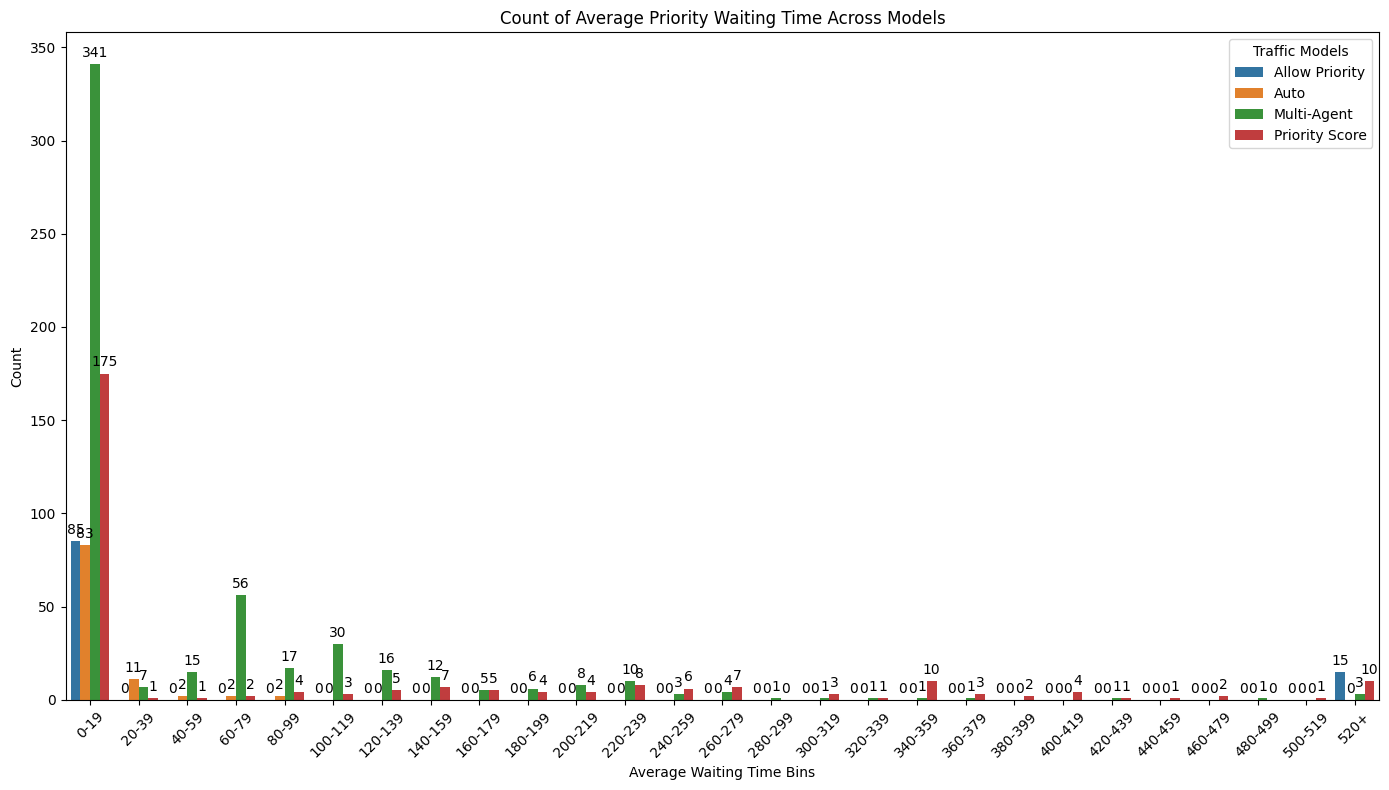
\includegraphics[width=1\linewidth]{images/count-average-priorirty.png}
    \caption{Priority Average Waiting Time  Distribution Across Models}
    \label{fig:setup}
\end{figure*}


\end{document}
